\documentclass[titlepage,12pt,a4paper]{article}
\usepackage[a4paper]{geometry}
\usepackage{amsmath}
\usepackage{amssymb}
\usepackage{enumitem}
\usepackage{commath}
\usepackage{mathtools}
\usepackage{graphicx}
\usepackage{dirtytalk}
\usepackage{csquotes}
\usepackage{hyperref}
\usepackage{tabto}
\usepackage{gensymb}
\usepackage{graphicx}
\usepackage{listings}
\usepackage{sidecap}

\usepackage{color}
\definecolor{dkgreen}{rgb}{0,0.6,0}
\definecolor{gray}{rgb}{0.5,0.5,0.5}
\definecolor{mauve}{rgb}{0.58,0,0.82}

\lstset{frame=tb,
  language=C++,
  aboveskip=3mm,
  belowskip=3mm,
  showstringspaces=false,
  columns=flexible,
  basicstyle={\small\ttfamily},
  numbers=left,
  numberstyle=\footnotesize,
  stepnumber=1,
  numbersep=5pt,
  keywordstyle=\color{blue},
  commentstyle=\color{dkgreen},
  stringstyle=\color{mauve},
  breaklines=true,
  breakatwhitespace=true,
  tabsize=3
}

\usepackage{fancyhdr}
\setlength{\headheight}{15.2pt}
\pagestyle{fancy}
\fancyhf{}
\lhead{ \fancyplain{}{COMP3431: Robotic Software Architecture} }
\rfoot{ \fancyplain{}{\thepage} }


\begin{document}
\begin{titlepage}
    \begin{center}
        \vspace*{3cm}
        
        \Huge
        \textbf{COMP3431\\}
        \title{}
        \vspace{0.5cm}
        \Huge
        \textbf{Robotic Software Architecture}
        
        \vspace{0.54cm}
        
        \Large
        Assignment 1: Report
        
        \vspace{5cm}

	\normalsize
	Christopher Manouvrier\\
	Aaron Ramshaw\\
	Simon Robilliard\\
	Oliver Tan\\
	Aneita Yang
        
	\vfill
        
        \Large
        September 5, 2015
        
    \end{center}
\end{titlepage}

\pagebreak

\section*{Exploration}

Before it can visit beacons in a specified order, the TurtleBot must first explore the maze to generate a map. In this assignment, FastSLAM is used, for its speed and accuracy, to generate the map. Although HectorSLAM produces a higher resolution map (0.01), FastSLAM's 0.05 resolution is sufficient for our purposes.\\
\\
A wall-follower, although guaranteed to map out the entire maze correctly, has limitations in its speed. It often spends more time than is necessary to finish mapping a location, following any walls it comes across, regardless of any existing knowledge about the area.\\
\\
To speed up the exploration of the unknown maze, a frontier-based search is performed on any existing data we have of the maze. This data is delivered to us in the form of an OccupancyGrid message, which publishes an array of integers from -1 to 100 representing knowledge of the maze. The search during the exploration phase looks for the closest frontier of -1s in the OccupancyGrid and the TurtleBot is then instructed to explore this closest frontier.\\
\\
TODO: Add maths/equations here\\
\\
To prevent the TurtleBot from crashing into walls, any walls that are detected during the Bot's exploration are "fattened" by 20cm. Given that the Bot's radius is 15cm, this gives the robot a 5cm leeway from the walls, and a 60cm-wide pathway to travel along. To "fatten" the walls, we occupy the rings of cells surrounding every wall in the current OccupancyGrid (Figure 1). Fattening the walls also blocks any gaps between the walls that the robot may have originally seen through.\\
\\
\pagebreak

\begin{figure}
	\centering
	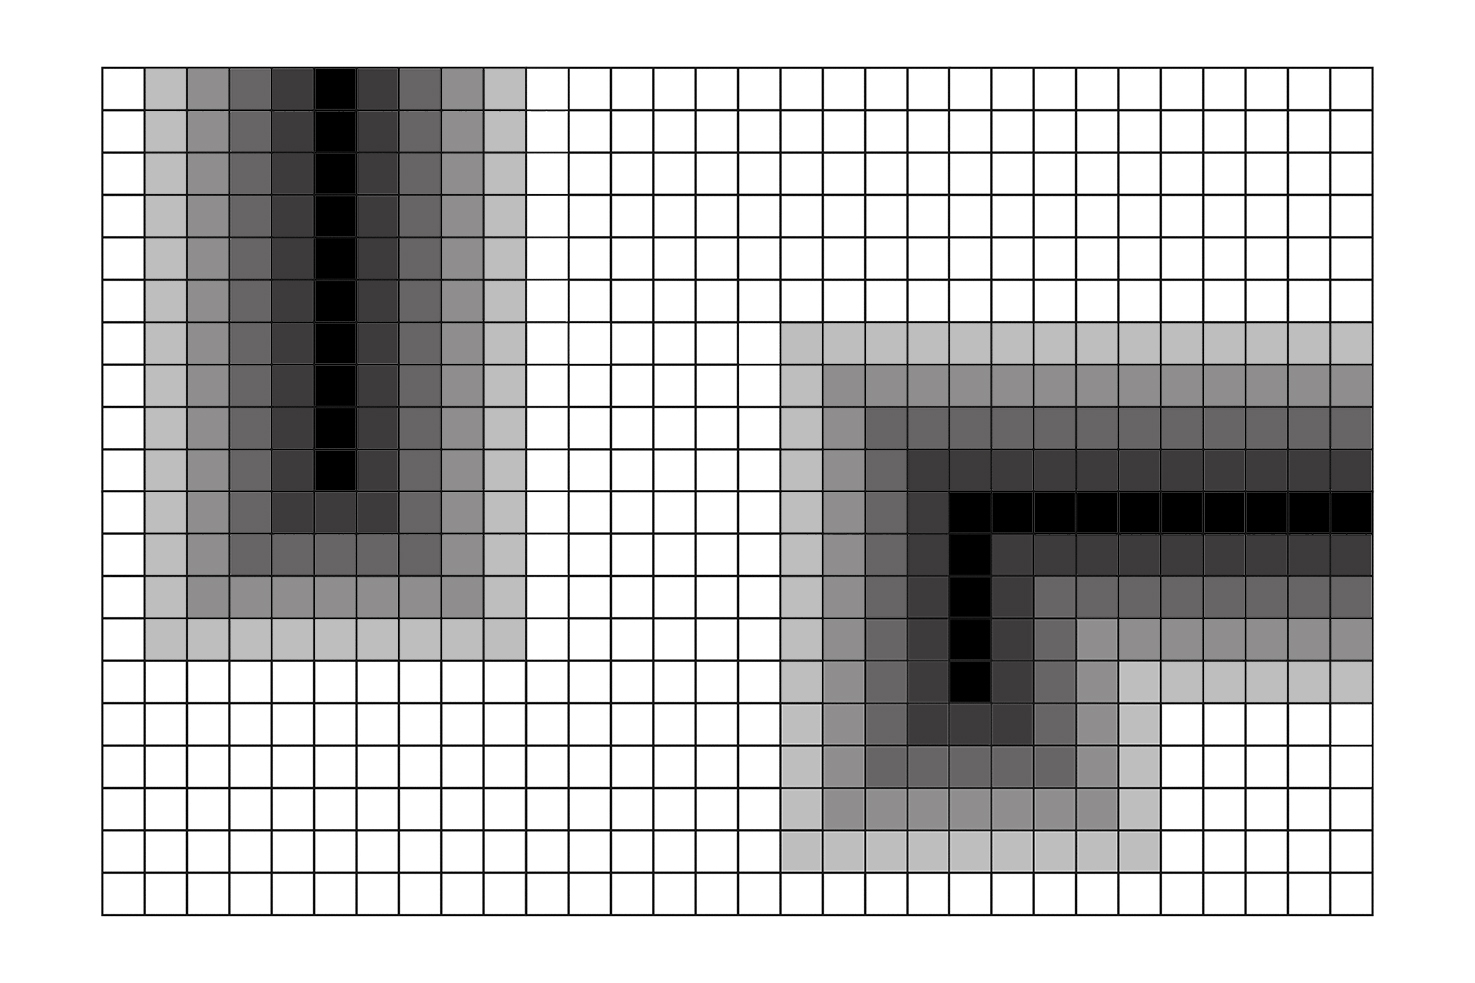
\includegraphics[scale=0.28]{wallfatten.jpg}
	\caption{Example of wall fattening by 4 cells, where black is the original wall}
\end{figure}

\begin{SCfigure}
	\centering
	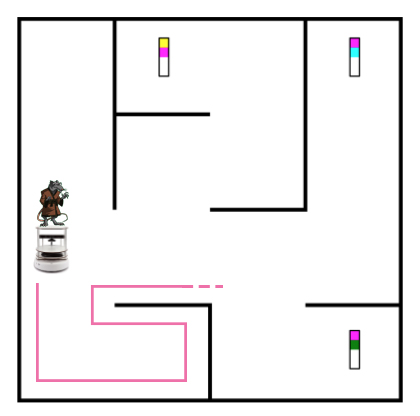
\includegraphics[scale=0.5]{wallfollowpath.jpg}
	\caption{Example of wall following exploration in a dead-end}
\end{SCfigure}

\begin{SCfigure}
	\centering
	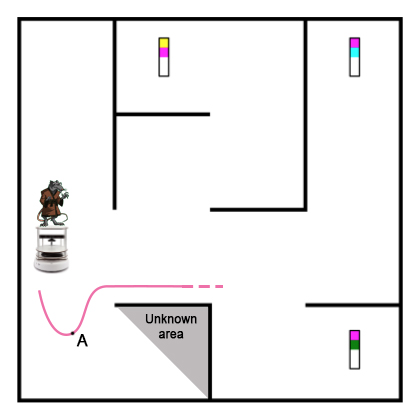
\includegraphics[scale=0.5]{searchpath.jpg}
	\caption{Example of frontier-based exploration in a dead-end. At point A, the robot will have seen all points in the dead end that were previously unknown.}
\end{SCfigure}

\pagebreak

\noindent 
\\
As the OccupancyGrid is continually being updated, our frontier-based search increases the speed of the search by eliminating the need for the TurtleBot to travel down dead-ends. Whereas a wall-follower would lead the Bot into the dead-end (Figure 2), the frontier-based search will not (Figure 3).\\
\\
As our frontier-based search is performed on a map with a resolution of 0.05, the path can often be jagged and over-complicated. In order to "smooth" our path, the Ramer-Douglas-Peucker algorithm is used to reduce the number of intermediary points in the path (see Appendix). RDP works by recursively dividing a given path, finding an intermediary point that is the furthest from the line segment drawn from the start to the end of a path. If the distance of this furthest point is within the given threshold, the point can be discarded, thus, cutting down the number of intermediary points the TurtleBot must visit. A threshold of 0.05 is used in our RDP path simplification, meaning that points that lie within 5cm can be overlooked.\\


\pagebreak


\section*{Beacon Recognition and Localisation}

\large{\textbf{\\Detection}} \\
\normalsize
\\
During the TurtleBot's first exploration of the maze, the camera is used to identify and position beacons. For every image frame captured by the Bot, we generate four additional images (for pink, yellow, blue and green), which only display the regions that lie within their colour thresholds. OpenCV's SimpleBlobDetector is used to extract the colour "blobs" from our images.\\
\\
To minimise the number of false positives and to distinguish between beacons and background colour noise, the SimpleBlobDetector filters by area, inertia and convexity and looks for areas in an image which satisfy the following criteria:

	\begin{enumerate}
		\item Area of the coloured region in the image is at least 200 pixels.
		\item Inertia of the detected region is greater than 0.65.
		\item Detected blob has a minimum convexity of 0.5.\\
	\end{enumerate}

\noindent
OpenCV's drawKeypoints is used to retrieve the location, as pixel values, of each detected colour region within an image. We conclude that a beacon has been successfully detected if there are two "blobs" in the same image frame within a 20 pixel offset from each other in the horizontal axis. This threshold of 20 pixels is used to account for any motion blur. The beacon's top colour is determined by comparing the two keypoints' y values.\\
\\
\large{\textbf{\\Localisation}} \\
\normalsize
\\
Pinpointing the locations of detected beacons is essential in order for the TurtleBot to complete Waypoint Traversal. Each beacon's position is determined by first considering the TurtleBot's position and orientation in the maze (i.e. relative to the origin of the map), and looking at data from the DepthCloud. \\
\\
To determine the rotation of the beacon from the origin of the map, we consider the pixel in the image at which the beacon was detected, relative to the centre pixel of the image. It is known that the camera has a 55\degree field-of-view and, thus, we are able to use these pixel values to calculate the beacon's rotation from the origin. \\
\\
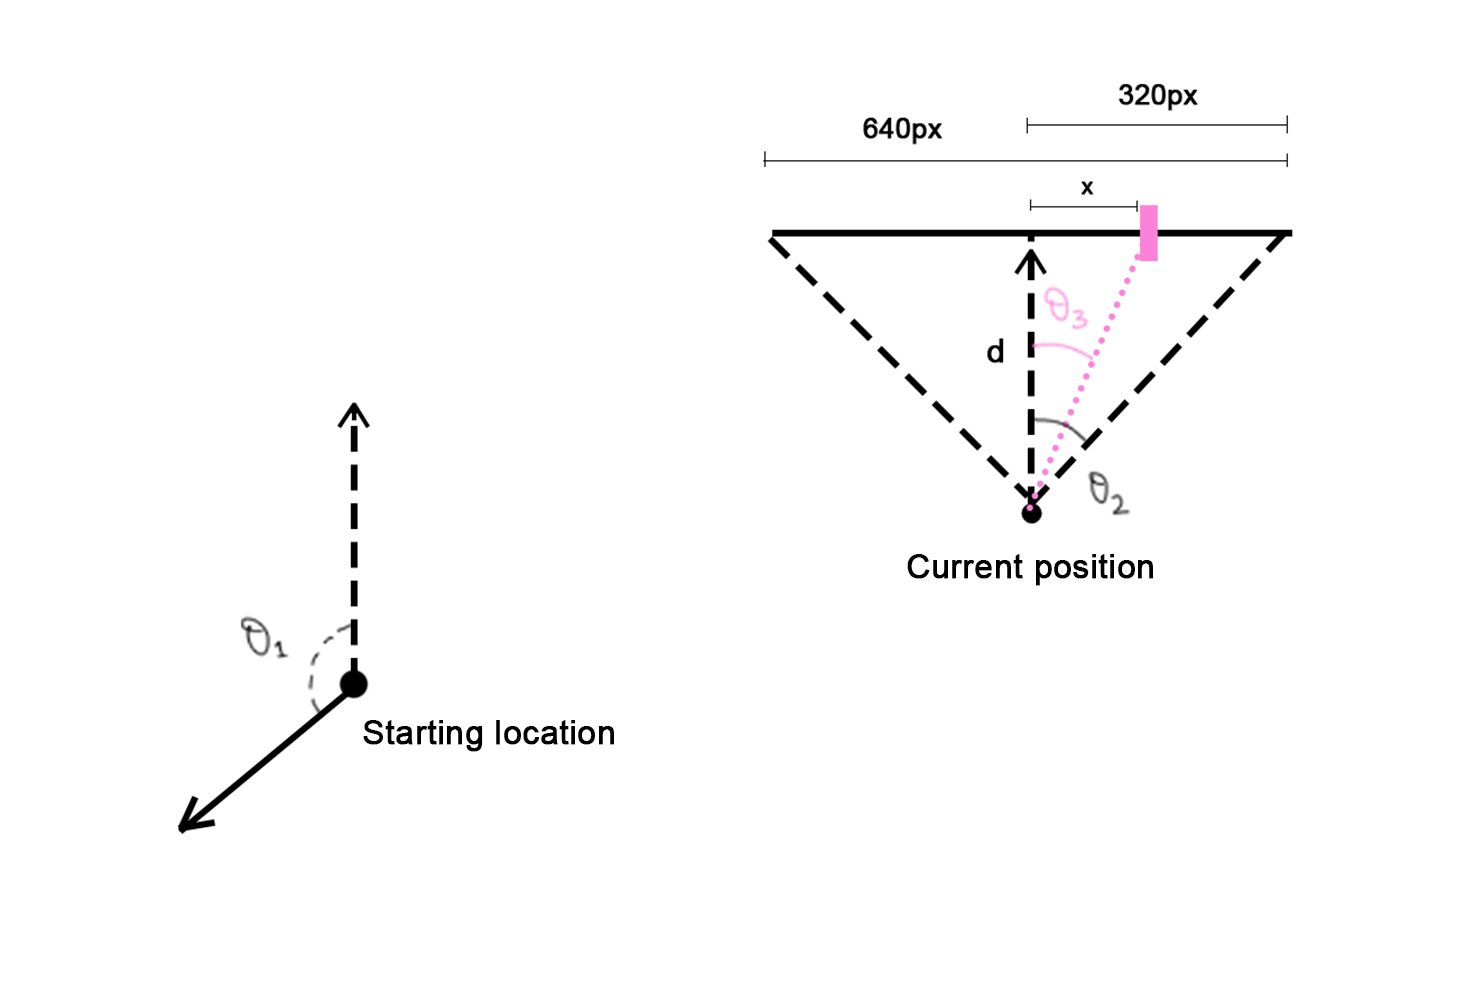
\includegraphics[scale=0.3]{beacon.jpg}

\begin{align*}
	\theta_1   &=  \text{TurtleBot's current yaw, relative to start} \\
	\theta_2   &=  27.5\degree \\
	\\
	a 	        &=  \frac{320}{\tan{27.5\degree}} \\ 
	b 	        &=  \text{position of beacon given as an offset from centre of image} \\
			&=  \text{vertical pixel in image at which beacon was detected} - 320\text{px} \\
	\\
	\theta_3   &= \tan^{-1}{(\frac{x}{d})} \\
\end{align*}
\\
Therefore, the beacon's yaw from the TurtleBot is $\theta_3$ and the beacon's yaw from the origin of the map is $\theta_1 + \theta_3$. Note that in the above example, $\theta_3$ is negative as tan is negative in the fourth quadrant.\\
\\
To determine the beacon's x and y coordinates in the map, we consider the TurtleBot's position, the beacon's angle from the TurtleBot ($\theta_3$), and the array of ranges gathered from the laser scan. \\
\\
\begin{align*}
	\text{beacon.x}		&=		\text{bot.x} + d \cdot \cos{(\theta_1 + \theta_3)} \\
	\text{beacon.y} 		&= 		\text{bot.y} + d \cdot \sin{(\theta_1 + \theta_3)} \\
	\\
	\text{where } d 		&=		\text{beacon's distance from TurtleBot} \\
					&=		\text{laser.ranges [angle of beacon in laser scan]}  \\
\end{align*}
\\
Using the ranges from the laser scan eliminates the need for the TurtleBot to be next to the beacon to pinpoint its location. Rather, once a beacon is within the camera's view, it's position can be determined, speeding up the process of beacon localisation. In turn, the TurtleBot's initial exploration is also sped up.


\pagebreak


\section*{Planner}

A vector of four Beacon objects is created when the beacon recognition module first begins, where the first index holds the first beacon to visit, the second index holds the second beacon to visit, and so on. Beacon objects store the top and bottom colour of the beacon as strings, x and y coordinates, and a boolean value as to whether the beacon has been found within the maze. \\
\\
As beacons are detected during the exploration phase, their positions are stored in the vector. Once the four beacons have been found, their coordinates are moved from the vector to a FoundBeacons message which is published, signalling to the Exploration module to stop and the Waypoint Traversal module to begin.\\
\\
This essentially allows our TurtleBot to stop exploring the maze once all four beacons have been detected, even if the full map of the maze has not been generated.\\
\\
\textbf{Beacon Class:}
\begin{lstlisting}
	class Beacon {
	public:
    		double x, y;
    		bool known_location;
    		string top, bottom;

    		Beacon(string top, string bottom) :
        			x(0), y(0),
        			known_location(false),
        			top(top), bottom(bottom) {}

    		bool found() {
        			return known_location;
    		}
	};
	
\end{lstlisting}

\textbf{\\FoundBeacons Message:}
\begin{lstlisting}[language=C++]
	int32 n
	geometry_msgs/Point[] positions
\end{lstlisting}


\pagebreak


\section*{Waypoint Traversal}

Once the maze has been successfully mapped and the positions of all beacons has been detected, the TurtleBot's next task is to visit the specified beacons in order. To speed up this process, an A* search is performed on the available data - namely, the OccupancyGrid and the FoundBeacons message.\\
\\
The A* search returns the path (as cells) from the TurtleBot's current location to it's goal.
\\
- Heuristic: Euclidean distance \\
- RDP algorithm to smooth out path


\pagebreak


\begin{lstlisting}[language=C++]
Path rdp_simplify (Path in, double threshold) {
    Path out;
    if (in.size() > 2) {
        // Find the vertex farthest from the line defined by 
        // the start and and of the path
        double max_dist = 0;
        size_t max_dist_i = 0;

        Line line = make_pair(in.front(), in.back());

        for (size_t i = 0; i < in.size(); i++) {
            double dist = distance_line_point(line, in[i]);
            if (dist > max_dist) {
                max_dist = dist;
	        max_dist_i = i;
             }
        }

        // If the farthest vertex is greater than our threshold,
        // we need to partition and optimize left and right
        if (max_dist > threshold) {
            // Partition 'in' into left and right subvectors,
            // and optimize them
            Path left, right;

            for (size_t i = 0; i < max_dist_i + 1; i++) {
                left.push_back(in[i]);
            }
            for (size_t i = max_dist_i; i < in.size(); i++) {
                right.push_back(in[i]);
            }

            Path leftSimplified = rdp_simplify(left, threshold);
            Path rightSimplified = rdp_simplify(right, threshold);

            // Stitch optimized left and right into 'out'
            out.clear();
            for (size_t i = 0; i < leftSimplified.size(); i++) {
                out.push_back(leftSimplified[i]);
            }
            for (size_t i = 1; i < rightSimplified.size(); i++) {
                out.push_back(rightSimplified[i]);
            }
        } else  {
            out.push_back(line.first);
            out.push_back(line.second);
        }
        return out;
    } else {
        return in;
    }
}
	
\end{lstlisting}


\end{document}